\chapter{Fundamentação Teórica}
\label{cap:fundamentacao}

Nesta seção são detalhados fundamentos teóricos necessários para compreensão da pesquisa. Inicialmente é discorrido sobre o sensoriamento empregado, tipos de sensores, valores aferidos, entre outras características. Posteriormente, é apresentado o modelo matemático \textit{Quarter Car} (QC), o qual descreve as mecânicas veiculares envolvidas no sistema de suspensão. Em seguida, são detalhadas as técnicas de IA utilizadas com o intuito de reconhecer e classificar os padrões de percepção veicular, dentre técnicas \textit{Machine Learning} clássico e \textit{Deep Learning}. Por fim, são apresentadas as métricas de avaliação adotadas.

\section{Sensoriamento}

Nesta seção, são apresentados os sensores inerciais, os quais constituem fonte principal de dados do estudo. Em seguida, é discorrido sobre o sensor magnetômetro e GPS, uma vez que servem como sensores auxiliares, comumente utilizados em conjunto com os inerciais para prover informações adicionais. 

\subsection{Sensores Inerciais}

Os sensores inerciais constituem dispositivos que produzem sinais através do princípio da inércia \cite{Braga2017}. Estes sensores compreendem acelerômetros e giroscópios, de um ou mais eixos \cite{Beeby2004}. O acelerômetro mede a força de aceleração (em $m/s^2$ ou $g$), enquanto  o giroscópio afere a taxa de rotação (em graus/segundo ou radianos/segundo), ambos sem a necessidade de um referencial externo \cite{Groves2013}. Sendo assim, a partir de um quadro de referência ou posição inicial destes sensores, forças externas que atuam sobre eles causam acelerações e mudanças de orientação (rotação) em um ou mais de seus eixos \cite{Kempe2011}. Em síntese, são sensores que necessitam de movimento para produção de dados. Neste estudo, estes movimentos são resultantes das forças produzidas pela tração do veículo e pelas interações com o ambiente no qual ele trafega.

\subsection{Magnetômetro}

O magnetômetro é um sensor auxiliar comumente embarcado com os sensores inerciais em um mesmo módulo. Este sensor, também de abordagem passiva, mede o campo geomagnético ambiental (em $\mu$T) em seus três eixos físicos \cite{Sattar2018}. Sendo assim, é geralmente aplicado junto aos ângulos de Euler para dar orientação aos dados, reorientando para o referencial da terra. Também é empregado em conjunto com os dados de aceleração para estimar a localização e velocidade mais rapidamente, uma vez que a taxa de amostragem do GPS é muito mais lenta que a dos sensores inerciais.

\subsection{Global Position System}

O Sistema de Posicionamento Global (\textit{Global Positioning System} - GPS) consiste de um sistema de satélites que orbitam o planeta, auxiliando receptores em terra a determinar sua localização \cite{Milette2012}. Sendo assim, além dos dados geodésicos de latitude e longitude, o receptor GPS também afere a velocidade do objeto que contém o sensor. Embora preciso, este sistema possui uma taxa de amostragem baixa em relação aos demais sensores, cerca de 1Hz.

\section{Quarter Car}

O modelo matemático \textit{Quarter Car} (QC) descreve as variáveis da dinâmica veicular, conforme ilustra a \autoref{fig:quarter_car}. O modelo QC possui propriedades relacionadas a roda, suspensão e amortecimento. A propriedade de massa suspensa do veículo $m_s$, fica acima da suspensão e representa um quarto da massa veicular. A propriedade de massa não suspensa $m_u$, abaixo da suspensão, inclui a massa de uma roda e do sistema de suspensão conectado a ela. Entre as massas, existe uma suspensão feita de mola com uma taxa de suspensão $K_s$, e de um amortecedor com uma taxa de amortecimento $C_s$, os quais suportam a massa suspensa. Uma vez que a massa não suspensa está em contato direto com a superfície da pista, existe a rigidez do pneu e sua  capacidade de absorção representadas pela taxa de amortecimento do pneu $K_t$ \cite{Yafeai2019,Loizos2008}. Logo, uma força que parte da superfície da pista atingindo o pneu, será irradiada para todos estes componentes, onde será suavizada pelo deslocamento de massa suspensa $Z_s$ e da massa não suspensa $Z_u$, antes de chegar a parte superior do veículo.

\begin{figure}[h]
  \centering
  \caption{O modelo \textit{Quarter Car}}
   \label{fig:quarter_car}
   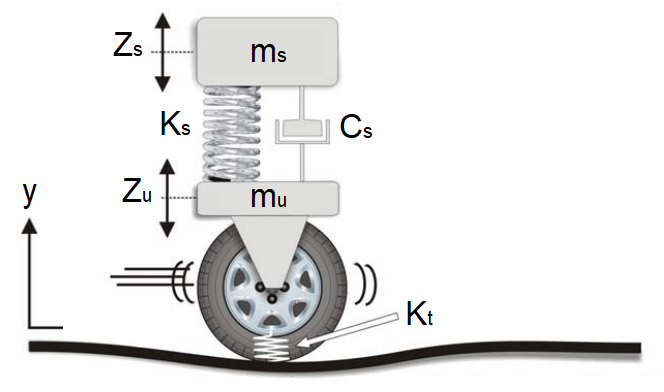
\includegraphics[width=0.8\textwidth]{figuras/fig_4.png}
   \fonte{Adaptado de \cite{Loizos2008}}
\end{figure}

Os valores das variáveis do modelo QC são definidos de acordo com cada veículo, dadas as diferentes estruturas veiculares existentes. Este modelo conta com diversas fórmulas que descrevem o relacionamento entre todas as suas variáveis. Os parâmetros do modelo são essenciais na aplicação de metodologias internacionais para indexação da irregularidade, como o IRI, para estabelecer a qualidade da via. De forma a simplificar as fórmulas do QC, foram criados valores padrões para as propriedades, denominados \textit{Golden Car Parameters}. Estas propriedades, detalhadas na \autoref{table:golden_car_parameters}, foram estabelecidas considerando um cenário padrão, onde o veículo é dirigido a uma velocidade constante de 80 $km/h$ \cite{Loizos2008}.

\begin{table}[h]
    \caption{Os parâmetros \textit{Golden Car}}
    \label{table:golden_car_parameters}
    \centering
    \small
    \begin{tabular}{cl}
        \toprule
        \textbf{Parâmetro} & \textbf{Valor} \\
        \toprule
        $K_s/m_s$ & 63,3 \\
        \midrule
        $K_t/m_s$ & 653 \\
        \midrule
        $C_s/m_s$ & 6 \\
        \midrule
        $m_u/m_s$ & 0,15 \\
        \bottomrule
    \end{tabular}
    \fonte{Adaptado de \cite{Loizos2008}}
\end{table}

\section{Técnicas Clássicas de Machine Learning}

Com o desenvolvimento da Inteligência Artificial, diversas técnicas surgiram para resolver problemas de classificação e regressão (previsão). Dentre as técnicas clássicas de \textit{clustering} e aprendizado de máquina supervisionado, neste trabalho foram desenvolvidos modelos de \textit{K-Means Clustering} (KMC), \textit{K-Nearest Neighbors} (KNN) e \textit{Support Vector Machines} (SVM), detalhadas nas próximas subseções.

\subsection{K-Means Clustering}

O KMC consiste de uma técnica não supervisionada para agrupamento de dados (\textit{clustering}), que permite identificar agrupamentos (\textit{clusters}) de dados semelhantes, conforme ilustra a \autoref{fig:execucao_kcm}. Neste método, partindo de um conjunto de dados não rotulados (1), são criadas aleatoriamente centróides para cada um dos \textit{k clusters} (2). Em seguida, cada dado é atribuído a um dos \textit{clusters} baseando-se em uma métrica de distância, como a Euclidiana, em relação ao centroide do \textit{cluster} (3, 4). Iterativamente, o centroide de cada \textit{clusters} é recalculado com base na média dos dados (5), e as distâncias novamente recalculadas (6, 7), até que as centroides sejam estabilizadas, ou o número máximo de iterações atingido \cite{foley2019,nisbet2009}.

\begin{figure}[h]
  \centering
  \caption{Execução da técnica KMC}
   \label{fig:execucao_kcm}
   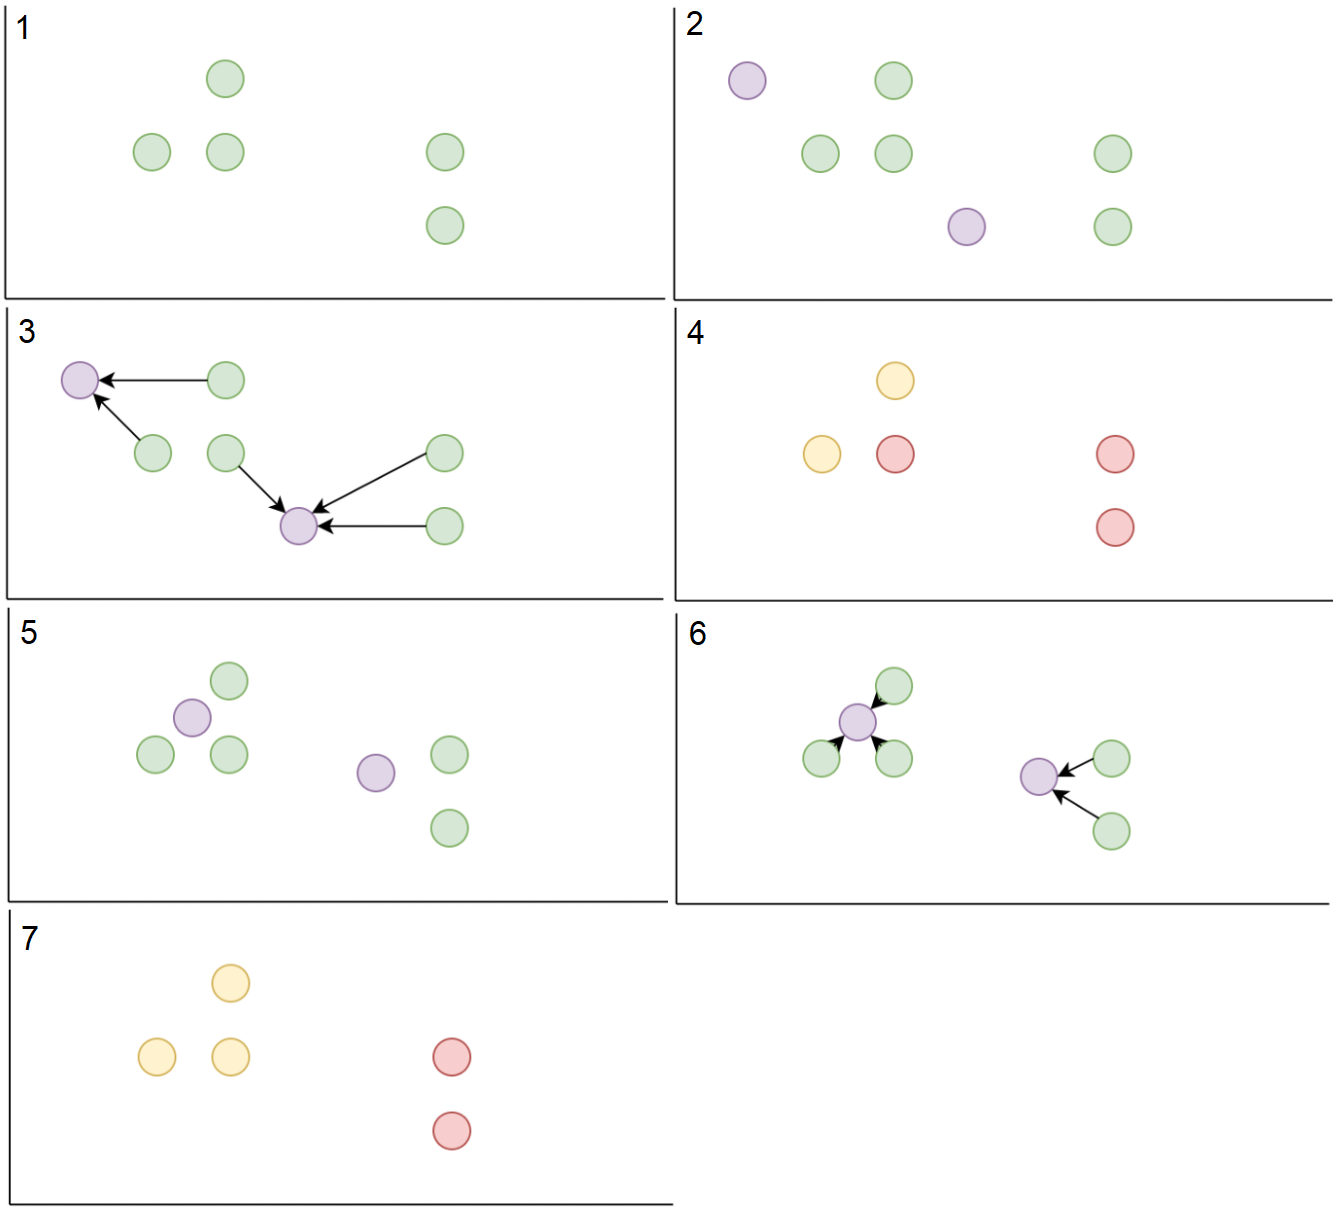
\includegraphics[width=0.7\textwidth]{figuras/fig_5.png}
   \fonte{Adaptado de \cite{i2020}}
\end{figure}

\subsection{K-Nearest Neighbors}

O KNN consiste de uma técnica para classificação a qual se baseia em métricas de similaridades entre os dados para reconhecer padrões. Desta forma, para um novo dado a ser classificado é calculada a distância entre ele e cada um dos dados de treinamento, identificando os $k$ vizinhos mais próximos. A classe do novo dado é definida como aquela mais comum entre seus $k$ vizinhos, conforme ilustra a \autoref{fig:execucao_knn} \cite{Khandelwal2018}.

\begin{figure}[h]
  \centering
  \caption{Execução da técnica KNN}
   \label{fig:execucao_knn}
   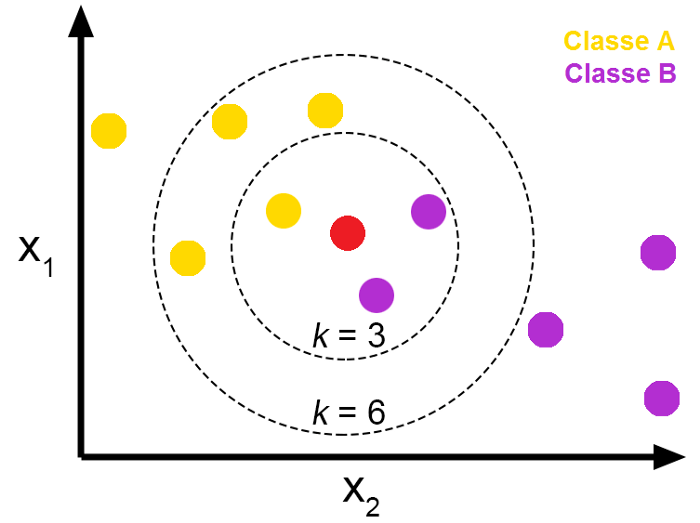
\includegraphics[width=0.4\textwidth]{figuras/fig_6.png}
   \fonte{\cite{Jose2018}}
\end{figure}

\subsection{Support Vector Machines}

O SVM é uma técnica de aprendizado supervisionado aplicada em classificação, onde se busca por um hiperplano ideal que separa as classes de dados, conforme ilustra a \autoref{fig:execucao_svm}. O algoritmo se inicia com a busca pelos pontos mais próximos ao hiperplano que separa as classes. Esses pontos são chamados de vetores de suporte. Na sequência, é calculada a distância entre o hiperplano e estes vetores. Essa distância é chamada de margem, a qual o SVM busca maximizar, de forma a encontrar o hiperplano ideal \cite{Pupale2019}. Em problemas não lineares, como é o caso deste, é necessário a utilização do hiperparâmetro \textit{kernel}, o qual converte problema não separável em problema separável, para que o SVM possa classificar \cite{Shubham2018}.

\begin{figure}[h]
  \centering
  \caption{Execução da técnica SVM}
   \label{fig:execucao_svm}
   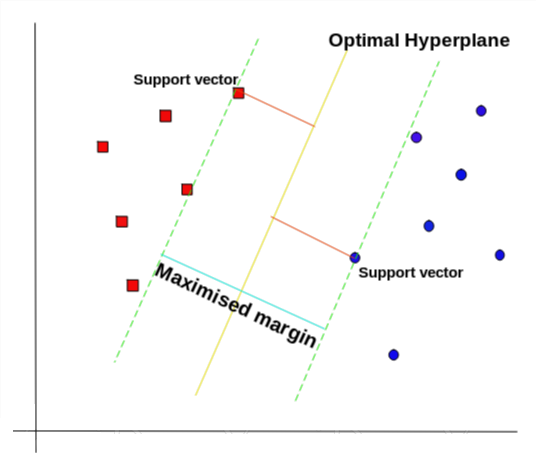
\includegraphics[width=0.7\textwidth]{figuras/fig_7.png}
   \fonte{\cite{Pupale2019}}
\end{figure}

\section{Técnicas de Deep Learning}

Com o desenvolvimento do aprendizado de máquina, especialmente a partir de 2006, surgiu nesta área um segmento denominado aprendizado profundo (\textit{Deep Learning}) \cite{Deng2014}. Até então, a extração características importantes que bem representassem os dados parametrizados à uma técnica de reconhecimento de padrões, constituía um problema central. Sendo assim, as técnicas existentes apresentavam a grande dificuldade de se extrair, em um pré-processamento, características de alto nível através de dados brutos \cite{Goodfellow2016}. 

Com o desenvolvimento do \textit{Deep Learning}, esse problema foi solucionado, sendo introduzidas representações que são expressas em termos de outras representações, construindo conceitos complexos através de conceitos simples \cite{Goodfellow2016}. Nessa abordagem, tornou-se possível construir modelos computacionais compostos de múltiplas camadas de processamento para aprender a representação dos dados com diversos níveis de abstração \cite{LeCun2015}. Sendo assim, o aprendizado profundo descobre uma estrutura complexa em grandes conjuntos de dados utilizando do algoritmo de retropropagação para calcular como alterar seus parâmetros internos, os quais são usados para estabelecer a representação em cada camada a partir da representação obtida na camada anterior \cite{LeCun2015}.

Com este novo paradigma, foram melhorados drasticamente o estado da arte em reconhecimento de fala, reconhecimento visual de objetos, detecção de objetos e muitos outros domínios \cite{LeCun2015}. Os diversos métodos presentes nessa categoria podem ser classificados entre redes profundas para aprendizado não supervisionado ou generativo, redes profundas para aprendizado supervisionado e redes profundas híbridas \cite{Deng2014}. Neste trabalho, foram utilizadas redes  profundas para aprendizado supervisionado do tipo \textit{Long Short-Term Memory} (LSTM), \textit{Convolutional Long Short-Term Memory} (ConvLSTM), \textit{Gated Recurrent Unit} (GRU)  e \textit{Convolutional Neural Network} (CNN), assim como redes profundas híbridas do tipo \textit{Convolutional Neural Network Long Short-Term Memory} (CNN-LSTM), discorridas nas próximas seções.

\subsection{Long Short-Term Memory}

A LSTM constitui um tipo de Rede Neural Recorrente (\textit{Recurrent Neural Network} - RNN) considerada ideal para predição e classificação de séries temporais, substituindo muitas abordagens tradicionais por \textit{Deep Learning} \cite{Zaccone2017}. Suas aplicações envolvem previsão ou classificação de séries temporais \cite{Zaccone2017}, tais como previsão de velocidade de tráfego, modelagem de linguagem, reconhecimento de fala, aprendizagem de gramática, modelagem de áudio, reconhecimento de caligrafia, etc. \cite{Bianchi2017}. Nesta abordagem, introduzindo o conceito de estado de célula (memória) e \textit{auto-loops} conforme ilustra a \autoref{fig:cell_lstm}, a rede pode manter valores por um curto ou longo período de tempo, como uma função de suas entradas. Assim, a célula consegue se lembrar daquilo que é importante, e não apenas do último valor computado \cite{Jones2017}, de forma que informações relevantes de entradas anteriores são retidas e utilizadas para alterar a saída atual \cite{Zebin2018}.

\begin{figure}[h]
  \centering
  \caption{Célula de uma LSTM com \textit{auto-loops}}
   \label{fig:cell_lstm}
   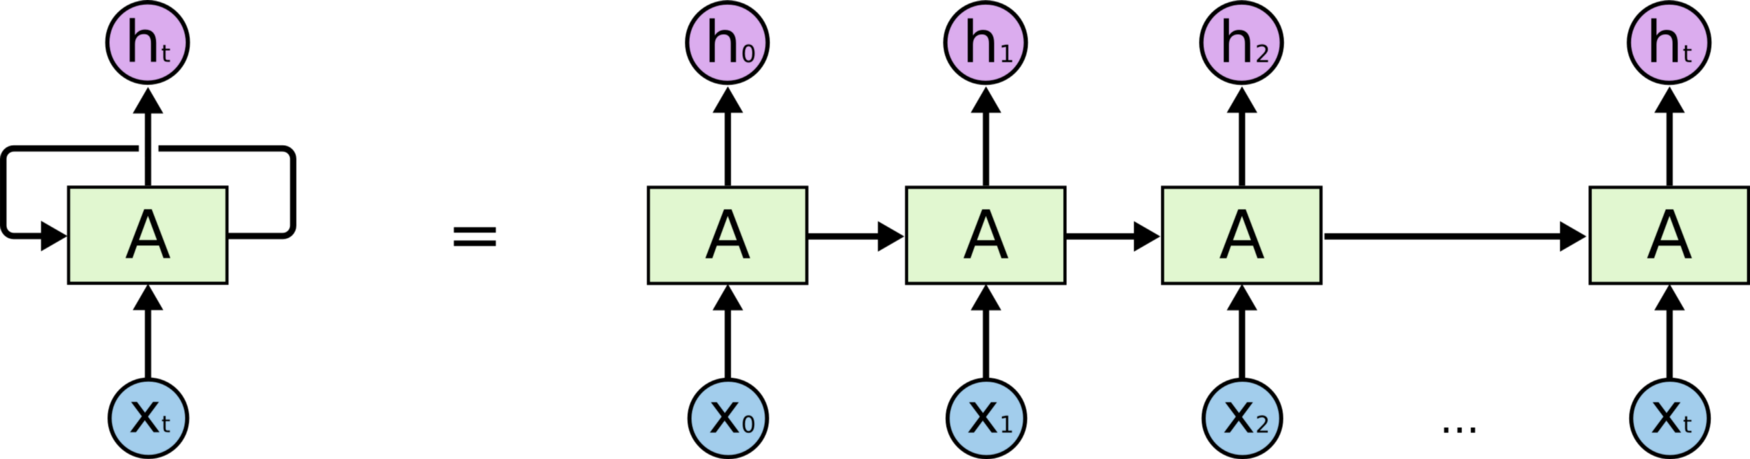
\includegraphics[width=0.8\textwidth]{figuras/fig_8.png}
   \fonte{\cite{Junior2019}}
\end{figure}

Cada célula de uma LSTM possui três portas que controlam o fluxo de informações para dentro e fora da célula, ilustrado na \autoref{fig:cell_lstm_gates}. Estas são: a porta de entrada (\textit{input gate}), a porta de saída (\textit{output gate}) e a porta de esquecimento (\textit{forget gate}). As portas possuem pesos, onde os valores computados seguem um fluxo no qual resultam em alterações no estado de célula. Sendo assim, inicialmente tem-se a porta de esquecimento, responsável por decidir quais dados devem ser mantidos na memória e quais devem ser esquecidos \cite{Phi2020}. Isso permite que a célula se lembre de dados anteriores importantes, ou apenas de novos dados, esquecendo os anteriores. Em seguida, a porta de entrada é responsável por controlar quando novas informações podem entrar na memória. Finalmente, a porta de saída controla quais as informações contidas no próximo estado da célula \cite{Jones2017}.

\begin{figure}[h]
  \centering
  \caption{Componentes de uma célula de LSTM}
   \label{fig:cell_lstm_gates}
   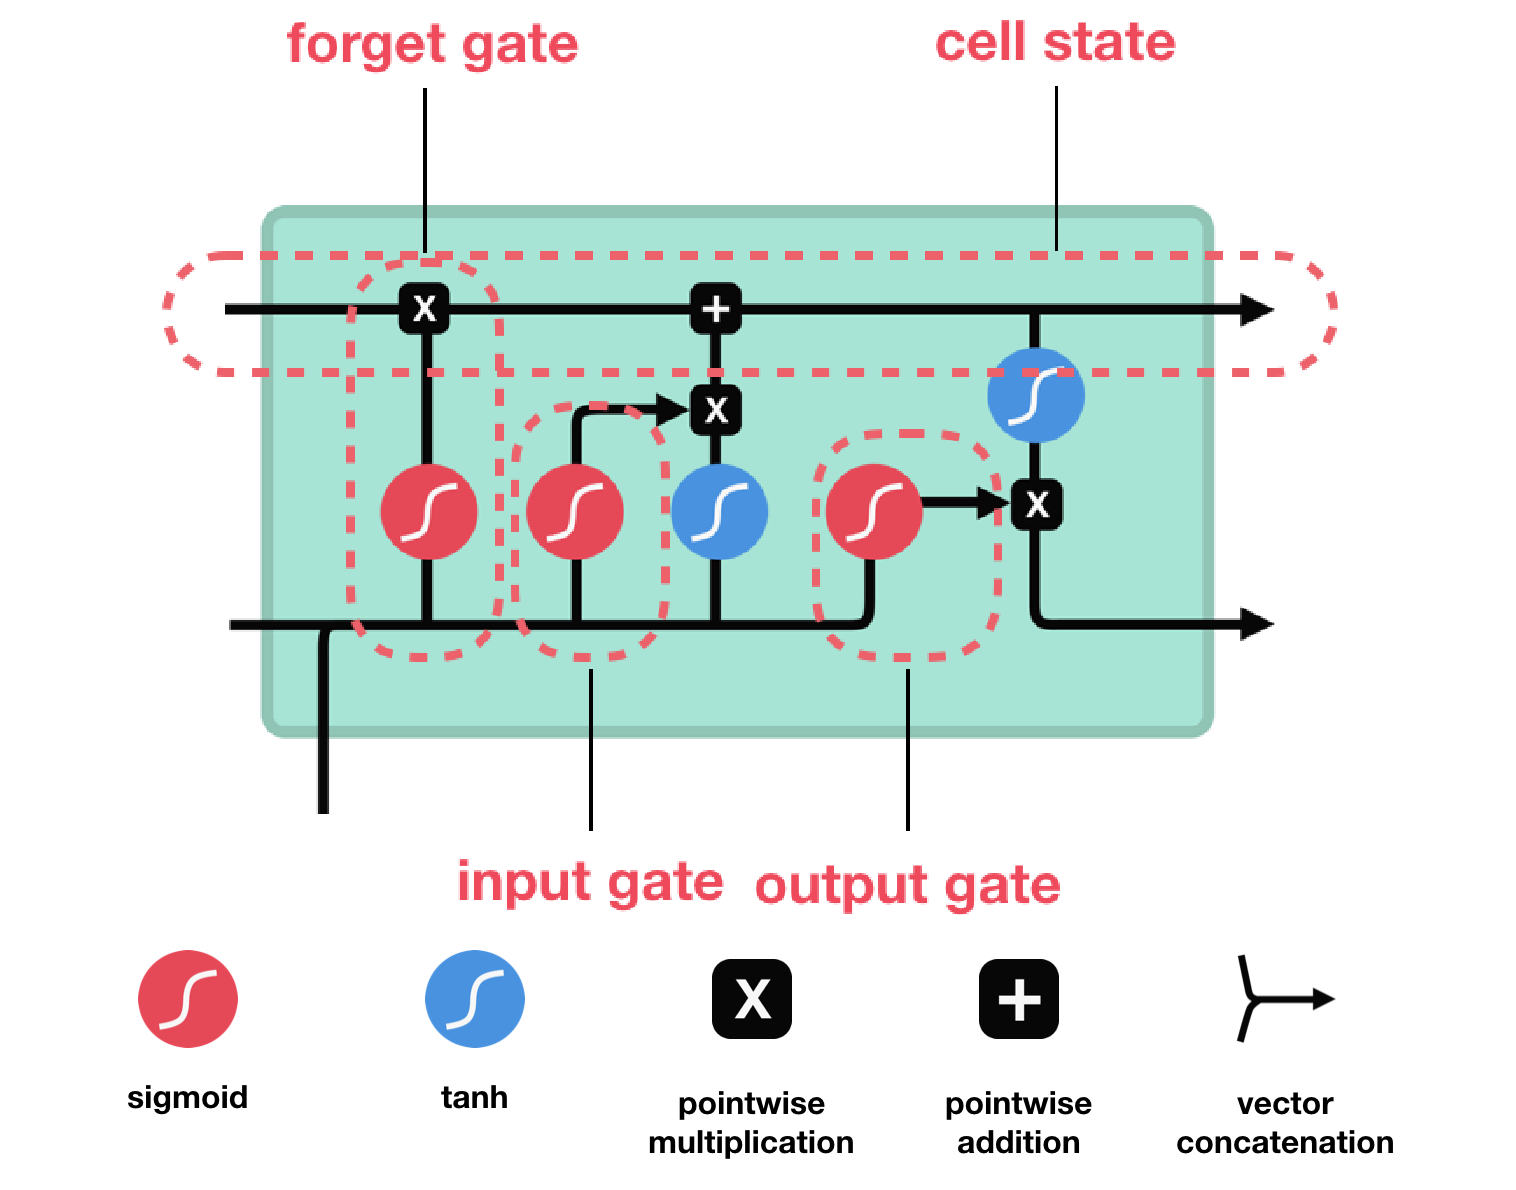
\includegraphics[width=0.8\textwidth]{figuras/fig_9.png}
   \fonte{Adaptado de \cite{Phi2020}}
\end{figure}

\subsection{Gated Recurrent Unit}

A GRU consiste de um tipo de RNN com o mesmo propósito da LSTM, embora considerada uma melhoria em relação a anterior, utilizando menos portas e parâmetros \cite{Kumar2019,Bianchi2017}. Em razão disso, redes GRU superaram a performance de redes LSTM em várias aplicações, treinando e convergindo mais rápido, se mostrando computacionalmente menos custosas e igualmente eficientes \cite{Kumar2019,Bianchi2017}. Empregada também em classificação e previsão de séries temporais, este tipo de rede ajuda na recuperação de informações em escalas de tempo distintas \cite{Bianchi2017,Kumar2019}. 

Cada célula de uma GRU possui um estado de célula (memória) que utiliza de um estado escondido (\textit{hidden state}) para transferir a informação, com é feito na LSTM. Contudo, a GRU utiliza de apenas duas portas, conforme ilustra a \autoref{fig:cell_gru_gates}: a porta de reinicialização (\textit{reset gate}) e a porta de atualização (\textit{update gate}). A porta de atualização opera de forma similar às portas de esquecimento e a de entrada de uma LSTM, decidindo quais informações descartar e quais informações novas adicionar a memória. A porta de reinicialização, por sua vez, é utilizada para decidir quais informações do passado devem ser esquecidas \cite{Phi2020}.

\begin{figure}[h]
  \centering
  \caption{Componentes de uma célula de GRU}
   \label{fig:cell_gru_gates}
   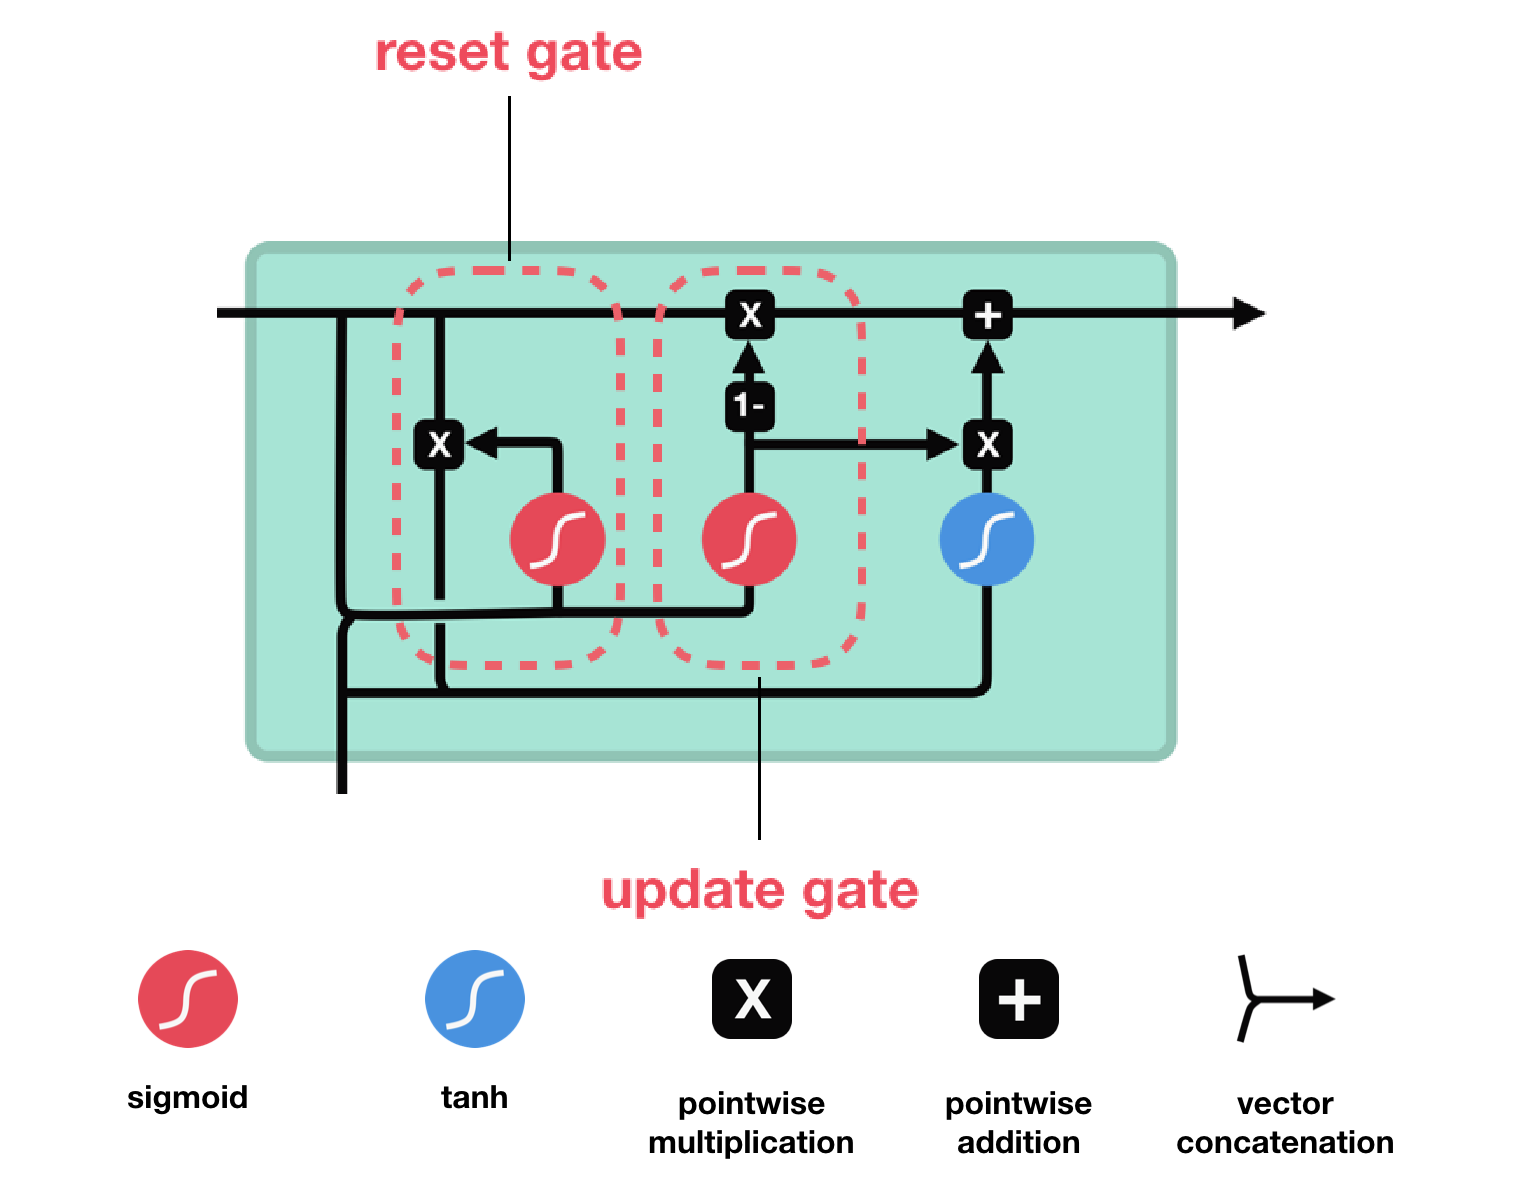
\includegraphics[width=0.8\textwidth]{figuras/fig_10.png}
   \fonte{Adaptado de  \cite{Phi2020}}
\end{figure}

\subsection{Convolutional Neural Network}

A CNN é um tipo de rede neural projetada para tratar eficientemente dados de imagem, se mostrando efetiva em aplicações de visão computacional, como classificação de imagem, localização de objetos, etc. \cite{Brownlee2018}. Através da aplicação de convoluções, este tipo de rede é capaz de aprender como extrair características de alto nível diretamente nos dados brutos, que representam bem os padrões a serem reconhecidos \cite{Dixon2019,Goodfellow2016}. Esta abordagem, denominada \textit{representation learning} \cite{Brownlee2018}, também pode ser aplicada em séries temporais, onde apresenta duas vantagens sobre outras técnicas: dependência local, uma vez que os sinais próximos provavelmente estão correlacionados; e invariância de escala para diferentes passos ou frequências \cite{Wang2019}. Neste tipo de rede, cada camada de convolução possui uma quantidade \emph{n} de filtros aplicados com um \textit{kernel} de tamanho \emph{m}, conforme ilustra as Figuras \ref{fig:cnn_convolution} e \ref{fig:cnn_convolution_3d}. Após a convolução, geralmente existem camadas de \textit{pooling} e \textit{fully connected}, que executam tarefas de classificação \cite{Wang2019}.

\begin{figure}[h]
  \centering
  \caption{Convolução em dados 1D}
   \label{fig:cnn_convolution}
   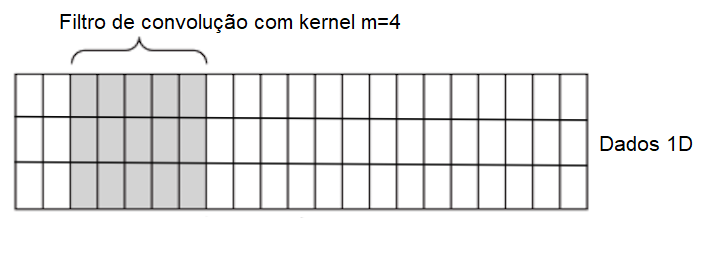
\includegraphics[width=0.9\textwidth]{figuras/fig_11.png}
   \fonte{\cite{Verma2020}}
\end{figure}

\begin{figure}[h]
  \centering
  \caption{Convolução em dados 3D}
   \label{fig:cnn_convolution_3d}
   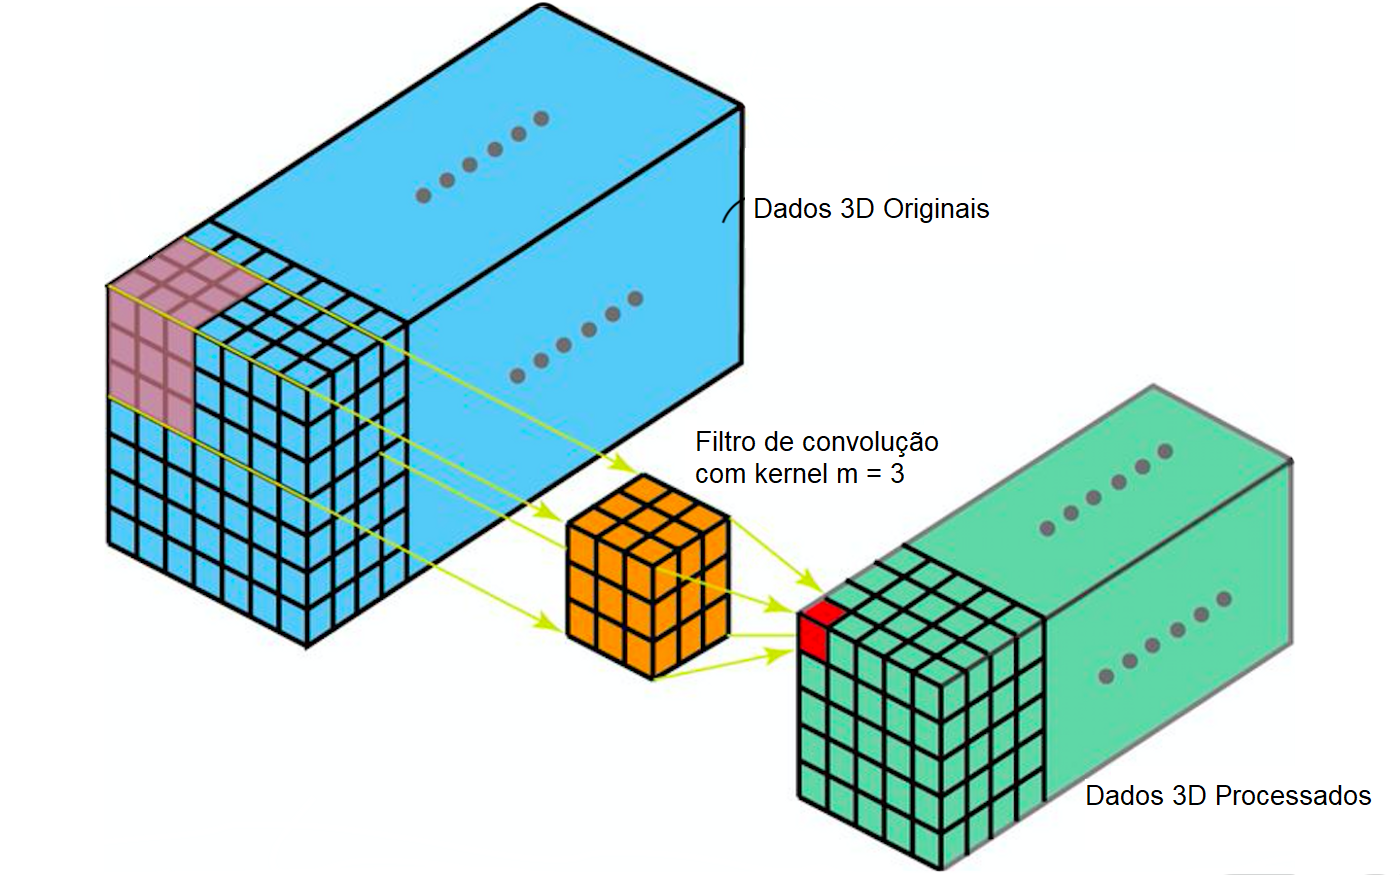
\includegraphics[width=0.8\textwidth]{figuras/fig_12.png}
   \fonte{\cite{Verma2020}}
\end{figure}

\subsection{Convolutional Long Short-Term Memory}

A ConvLSTM é um tipo de RNN variante da LSTM \cite{Salman2018}. Nestas redes existem operações de convolução dentro da célula de LSTM, de forma que as estruturas de convolução são aplicadas tanto na transição de entrada para estado, quanto nas transições de estado para estado. Desta forma, todas as operações de multiplicação de matrizes interna são substituídas por convoluções \cite{Rahman2019}. Neste ponto se mostra evidente a diferença para a híbrida CNN-LSTM, nas quais estruturas de convolução (CNN) são aplicadas como a primeira camada e sequencialmente na segunda camada é aplicada LSTM \cite{Rahman2019}.

\subsection{Convolutional Neural Network Long Short-Term Memory}

A CNN-LSTM constitui um tipo de rede neural híbrida que utiliza ambas as camadas de convolução (CNN) e recorrência (LSTM) \cite{Deep2019}. Nestas redes, os sinais são inicialmente agrupados em sequências temporais, e cada sequência é subdividida em blocos menores, as subsequências. Nestas subsequências são aplicadas camadas de convolução para extração de características complexas \cite{Deep2019}. Em seguida, estas características são agrupadas novamente na sequência original e empregadas em camadas recorrentes, para interpretar a sequência temporal das características produzidas.

\section{Métricas de Avaliação}

Para mensurar os resultados dos experimentos foram adotadas métricas comumente utilizadas em problemas de classificação: acurácia, precisão, \textit{recall} e \textit{f1-score} \cite{Rodrigues2020,Rodrigues2021,Shung2020}. Em um problema de classificação, os resultados podem ser classificados em Verdadeiros Positivos (VP), sendo a classificação correta da classe Positivo; Verdadeiros Negativos (VN), a classificação correta da classe Negativo; Falsos Positivos (FP), erro em que o modelo previu a classe Positivo quando o valor real era classe Negativo; e Falsos Negativos (FN), erro em que o modelo previu a classe Negativo quando o valor real era classe Positivo \cite{Rodrigues2020}. A \autoref{fig:classificacao_positivo_negativo} ilustra os resultados possíveis.

\begin{figure}[h]
  \centering
  \caption{Matriz confusão de classificação}
   \label{fig:classificacao_positivo_negativo}
   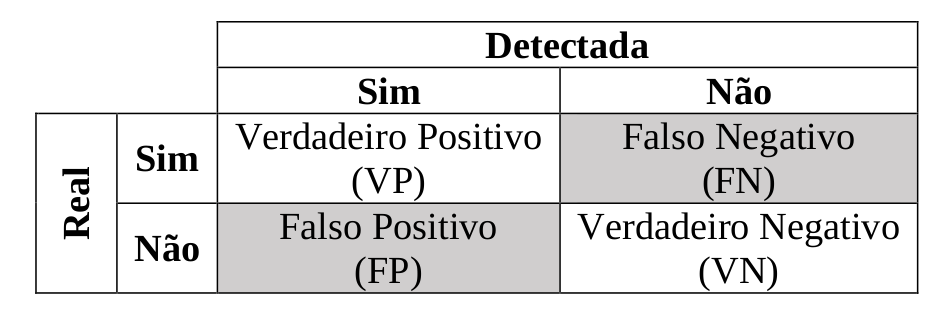
\includegraphics[width=0.6\textwidth]{figuras/fig_13.png}
   \fonte{\cite{Rodrigues2020}}
\end{figure}

A acurácia indica uma performance geral do modelo. Desta forma, consiste da proporção de amostras classificadas corretamente em relação ao total de amostras, considerando todas as classes de dados. A fórmula desta métrica é apresentada a seguir:

\begin{center}
  \[
  \textit{Acurácia} = \frac{VP + VN}{VP + VN + FP + FN}
  \]
\end{center}

Por outro lado, as métricas de precisão, \textit{recall} e \textit{f1-score} avaliam cada uma das classes de dados separadamente, de modo que se possa verificar problemas de desbalanceamento e viés. A precisão mede a proporção de amostras preditas corretamente em relação ao total de predições para determinada classe de dados, conforme a seguinte fórmula:

\begin{center}
  \[
  \textit{Precisão} = \frac{VP}{VP + FP}
  \]
\end{center}

A \textit{recall} mede a proporção de amostras preditas corretamente para determinada classe de dados em relação a todas as amostras reais daquela classe, conforme a seguinte fórmula:

\begin{center}
  \[
  \textit{Recall} = \frac{VP}{VP + FN}
  \]
\end{center}

Por fim, a \textit{f1-score} consiste da média harmônica de precisão e \textit{recall}, conforme a fórmula a seguir:

\begin{center}
  \[
  \textit{F1-Score} = \frac{2 \cdot \textit{precisão} \cdot \textit{recall}}{\textit{precisão} + \textit{recall}}
  \]
\end{center}
